\documentclass{standalone}
%\pagenumbering{gobble}


%%%%%%%%%%%%%%%%%%%%%%%%%%%%%%%%%%%%%%%%%%%%
% fluid element showing conservation of mass
%
%%%%%%%%%%%%%%%%%%%%%%%%%%%%%%%%%%%%%%%%%%%%


\usepackage{tikz,xcolor}
\usetikzlibrary{arrows,snakes}

\tikzset{
	partial ellipse/.style args={#1:#2:#3}{insert path={+ (#1:#3) arc (#1:#2:#3)}}
	}

\begin{document}


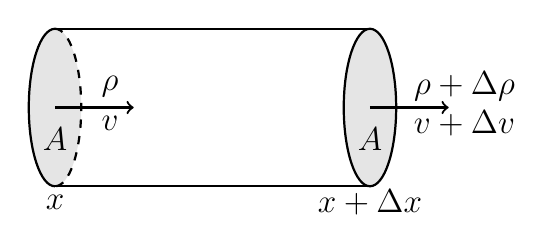
\begin{tikzpicture}[scale=1.0, font=\sffamily]

	% ellipse with dotted back side
	\draw[thick, fill=gray!20] (3,0) [partial ellipse=-90:90:-0.333 and 1];
	\draw[thick, dashed, fill=gray!20] (3,0) [partial ellipse=90:-90:0.333 and 1];
	% end of cylinder
	%\draw[thick] (7,0) ellipse (0.333 and 1);
	\draw[thick, fill=gray!20] (7,0) [partial ellipse=0:360:-0.333 and 1];

	% side of cylinder
	\draw[thick] (3,1) -- (7,1);
	\draw[thick] (3,-1) -- (7,-1);

	% arrows to show flow in and out
	%\draw[fill] (3,0) circle (0.1);
	%\draw[thick, line width=1mm, color=gray!50, ->] (3,0) -- (4,0);
	\draw[thick, ->] (3,0) -- (4,0);
	\draw[thick, ->] (7,0) -- (8,0);

	% annotation
	\node[align=center] at (3.7,0.27) {\large $\rho$};
	\node[align=center] at (3.7,-0.2) {\large $v$};
	\node[align=center] at (8.2,0.27) {\large $\rho+\Delta\rho$};
	\node[align=center] at (8.2,-0.2) {\large $v+\Delta v$};
	\node[align=center] at (3.0,-1.2) {\large $x$};
	\node[align=center] at (7.0,-1.2) {\large $x+\Delta x$};
	\node[align=center] at (3.0,-0.4) {\large $A$};
	\node[align=center] at (7.0,-0.4) {\large $A$};


\end{tikzpicture}

\end{document} 
